\subsection{Hyperflow}
\label{s:ProblemDomain:Hyperflow}

\emph{Workflow Management System (WMS)} is a software responsible for coordinating and supervising workflow execution.
It provides storage layers for data exchange, manages states of the workflow's tasks and handles permissions for waiting jobs to allow them to run only when their dependencies are fulfilled.
One of such systems is \emph{Hyperflow} -- an innovative yet lightweight and simple model for workflow execution \cite{b:Hyperflow}.
Its two main constituents are an engine, which makes all the decisions regarding workload allocation, and an executor that handles assigned workloads within separate processes, monitors their status and reports completion to the engine.


Executors are the supervisors spawned by an engine using a concept Hyperflow functions.
With each one implementing a different workload deployment solution for a specific kind of infrastructure Hyperflow can be used in various computing environments including Kubernetes clusters \cite{b:Hyperflow-k8s-deployment}.
The \cref{fig:hyperflow:architecture} presents an overview of a system architecture in a Kubernetes environment.
Each workflow's task is considered as a separate workload and is represented by a single Kubernetes job.
Its deployement is being requested by the Hyperflow engine through a function that calls the cluster's API.


%%%%
\begin{figure}[H]
\centering
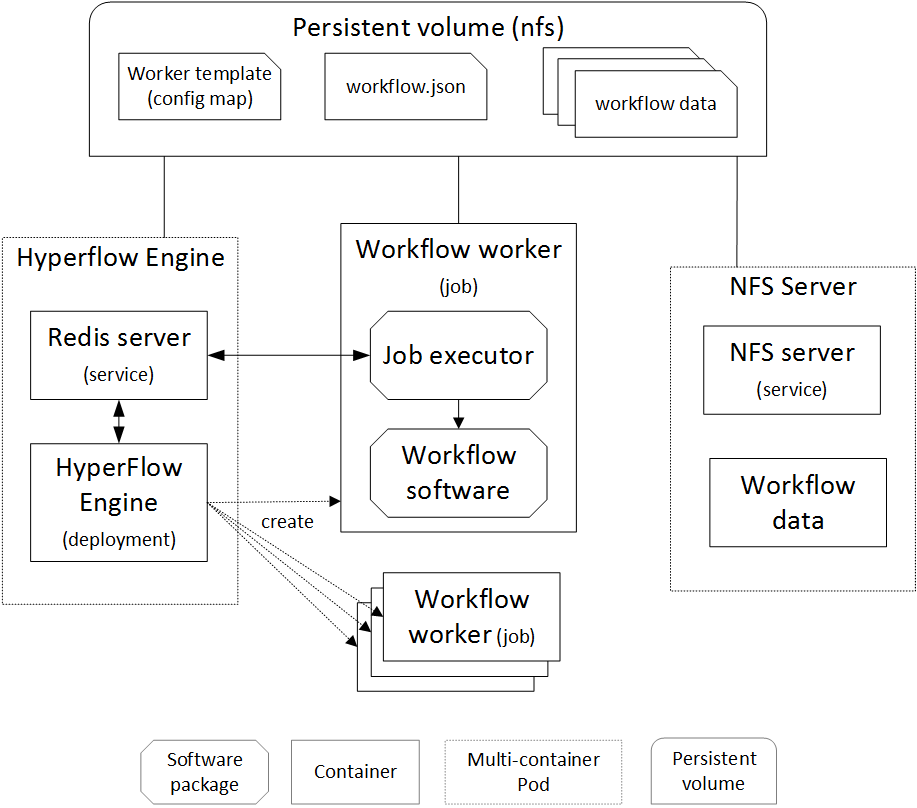
\includegraphics[width=0.6\linewidth]{figures/2-4-hyperflow-k8s-arch.png}
\caption{Hyperflow architecture in Kubernetes cluster}

\smallskip
\begin{minipage}{0.7\textwidth}
{\footnotesize\centering
SOURCE: \cite{b:Hyperflow-k8s-deployment}
\par}
\smallskip
{\footnotesize
One of the cluster's nodes is reserved to be a Hyperflow master node.
Engine's components are deployed on the master node, while tasks are deployed with their executors on the worker nodes.
Workflow data is being exchanged through network file system.
\par}
\end{minipage}

\label{fig:hyperflow:architecture}
\end{figure}
%%%%

The engine allows the tasks performing the same operations to be grouped together and buffered, waiting to be assigned to a single executor instance.
Whenever a task becomes ready to be processed it is being either assigned to a new buffer or is being appended to already existing one, associated with this specific task's operation.
This feature is an implementation of a horizontal task clustering solution and is referred to as \emph{task agglomeration} in Hyperflow nomenclature.

Buffers have configurable maximum sizes and have defined time boundaries for them to wait until they are deployed as a Kubernetes job.
They allow grouping until they are already full or the timeout has been reached.
Such configurations are possible for each workflow's operation.

